\section{The two-dimensional Case}\label{sec:two-d_case}
We take $\Omega$ to be a bounded open domain in $\mathbb{R}^2$ (assume that it is smooth for simplicity), and decompose $\Omega$ into two subdomains $\Omega_1$, $\Omega_2$ such that $\Omega=\Omega_1\cup\Omega_2$.

Consider the Neumann Problem
$$\begin{cases}
-\Delta u+u=f  \mbox{ in } \Omega, \\
\frac{\partial u}{\partial n}=0 \mbox{ on } \partial \Omega \\
\end{cases}$$
where $n$ is the outward pointing normal.

Let $X=H^{1}(\Omega)$,
and define 
$$Y_1:=\overline{\{\phi\in C^{\infty}(\Omega):\phi=0 \mbox{ in the neighbourhood of } \Omega\setminus \Omega_1\}}=H_{0}^{1}(\Omega_1),$$ and
$$Y_2:=\overline{\{\phi\in C^{\infty}(\Omega):\phi=0 \mbox{ in the neighbourhood of } \Omega\setminus \Omega_{2}\}}=H_{0}^{1}(\Omega_2).$$

Fix $u_0\in X$ and find $u_1$ by first solving
$$\begin{cases}
-\Delta u_1+u_1=f  \mbox{ in } \Omega_1, \\
u_1=u_0 \mbox{ on } \gamma_1:=\partial\Omega_1\cap\Omega_2 ,\\
\frac{\partial u_1}{\partial n}=0  \mbox{ on }\partial\Omega_1\setminus \gamma_1\\
\end{cases}$$ 
and then extend by $u_0$ from $\Omega_1$ to all of $\Omega$.
We repeat the procedure alternatingly to find $u_2,u_3,\cdots$ such that $u_{2n+1}$ (for $n\geq 0$) solves
$$\begin{cases}
-\Delta u_{2n+1}+u_{2n+1}=f  \mbox{ in } \Omega_1, \\
u_{2n+1}=u_{2n} \mbox{ on } \gamma_1:=\partial\Omega_1\cap\Omega_2 ,\\
\frac{\partial u_{2n+1}}{\partial n}=0  \mbox{ on }\partial\Omega_1\setminus \gamma_1\\
\end{cases}$$ 
while $u_{2n}$ (for $n\geq 1$) is a solution of 
$$\begin{cases}
-\Delta u_{2n}+u_{2n}=f  \mbox{ in } \Omega_2, \\
u_{2n}=u_{2n-1} \mbox{ on } \gamma_2:=\partial\Omega_2\cap\Omega_1 ,\\
\frac{\partial u_{2n}}{\partial n}=0  \mbox{ on }\partial\Omega_2\setminus \gamma_2\\
\end{cases}$$  
We may extend $u_{2n+1}$ by $u_{2n}$ and $u_{2n}$ by$u_{2n-1}$ respectively to all of $\Omega$.

Since $-\Delta(u_1-u)+(u_1-u)=0 \mbox{ in } \Omega_1$,$$\left\langle u_1-u,\phi\right\rangle_{H^1}=\int_{\Omega_1}(u_1-u)'\phi'+(u_1-u)\phi dx=\int_{\Omega_1}-(u_1-u)''\phi+(u_1-u)\phi dx=0$$ for all $\phi\in Y_1.$ This shows that $u_1-u\perp Y_1$. Let $M_i=Y_{i}^{\perp}$ for $i=1,2$, then $u_1-u\in M_1$. 

Note that $$u_0-u=(u_0-u_1)+(u_1-u)$$ where $u_0-u_1\in Y_1=M_{1}^{\perp}$ and $u-u_1\in M_1$, so $u_1-u=P_{1}(u_0-u)$ where $P_{i}$ is the orthogonal projection onto $M_i$ for $i=1,2$. 

Similarly, $u_2-u=P_{2}(u_1-u)$ as $$u_1-u=(u_1-u_2)+(u_2-u)$$ where $u_2-u\in M_2$ and $u_1-u_2\in M_{2}^{\perp}$.

Iteratively, $$u_{2n+1}-u=P_{1}(u_{2n}-u)$$ and $$u_{2n}-u=P_{2}(u_{2n-1}-u)$$ for $n\geq 1$.

Let $T=P_{2}P_{1}$. If $x_{2n}:=u_{2n}-u$, $x_0:=u_0-u$, then $x_{2n}=T^n x_0$.
By \emph{Von-Neumann Halperin Theorem}, $$\lim_{n\rightarrow \infty}\|T^n x_0-P_{M}x_0\|_{H^1}=0$$ where $M=M_1\cap M_2$. In this case, we have $$X=\overline{M_{1}^{\perp}+M_{2}^{\perp}}=\overline{Y_1+Y_2}(\star),$$ so $M=M_1\cap M_2=\{0\}$, and $P_{M}x_0=0$. Then $$\lim_{n\rightarrow \infty} \|x_{2n}\|_{H^1}=0.$$ This implies that $u_{2n}(x)$ converges to $u(x)$ strongly.

Note that $x_{2n+1}=P_{1}x_{2n}$, then
$$\lim_{n\rightarrow \infty}\|x_{2n+1}\|_{H^1}=\lim_{n\rightarrow \infty} \|P_{1}x_{2n}\|_{H^1}=0$$ by continuity of $P_{1}$. That is, $u_{2n+1}$ converges to $u$ strongly as well.

Thus, the \emph{Schwarz Alternating Method} generates a sequence of solutions $\{u_n\}$ converging to the exact solution $u$ strongly.
\par
The rate of convergence depends on whether $Y=Y_1+Y_2$ is closed by \emph{Von Neumann-Halperin Dichotomy}. If $Y$ is closed, that is, the closures of $\gamma_1$ and $\gamma_2$ have empty intersection \cite{PL88}, then convergence is exponentially  fast, and otherwise for each $(r_n)\in c_0$, $r_n\in\mathbb{R}^{+}$, for all $x\in X$, $\|T^n x-P_{M}x\|=\|T^n x\| \neq O(r_n)$.
\par
We formulate the proof of $(\star)$ in the following lemma:
\begin{lemma}
For $X=H^1(\Omega)$,$Y_i=\overline{Z_i}$ where $$Z_i:=\{u\in C^{\infty}(\Omega)\colon u=0 \mbox{ in the neighbourhood of } \Omega\setminus\Omega_1\},$$ 
$Y=Y_1+Y_2$ is a proper dense subspace of $X$.
\begin{proof}
For simplicity, we consider the two-dimensional domain $\Omega$ as shown below.
\begin{figure}[h]
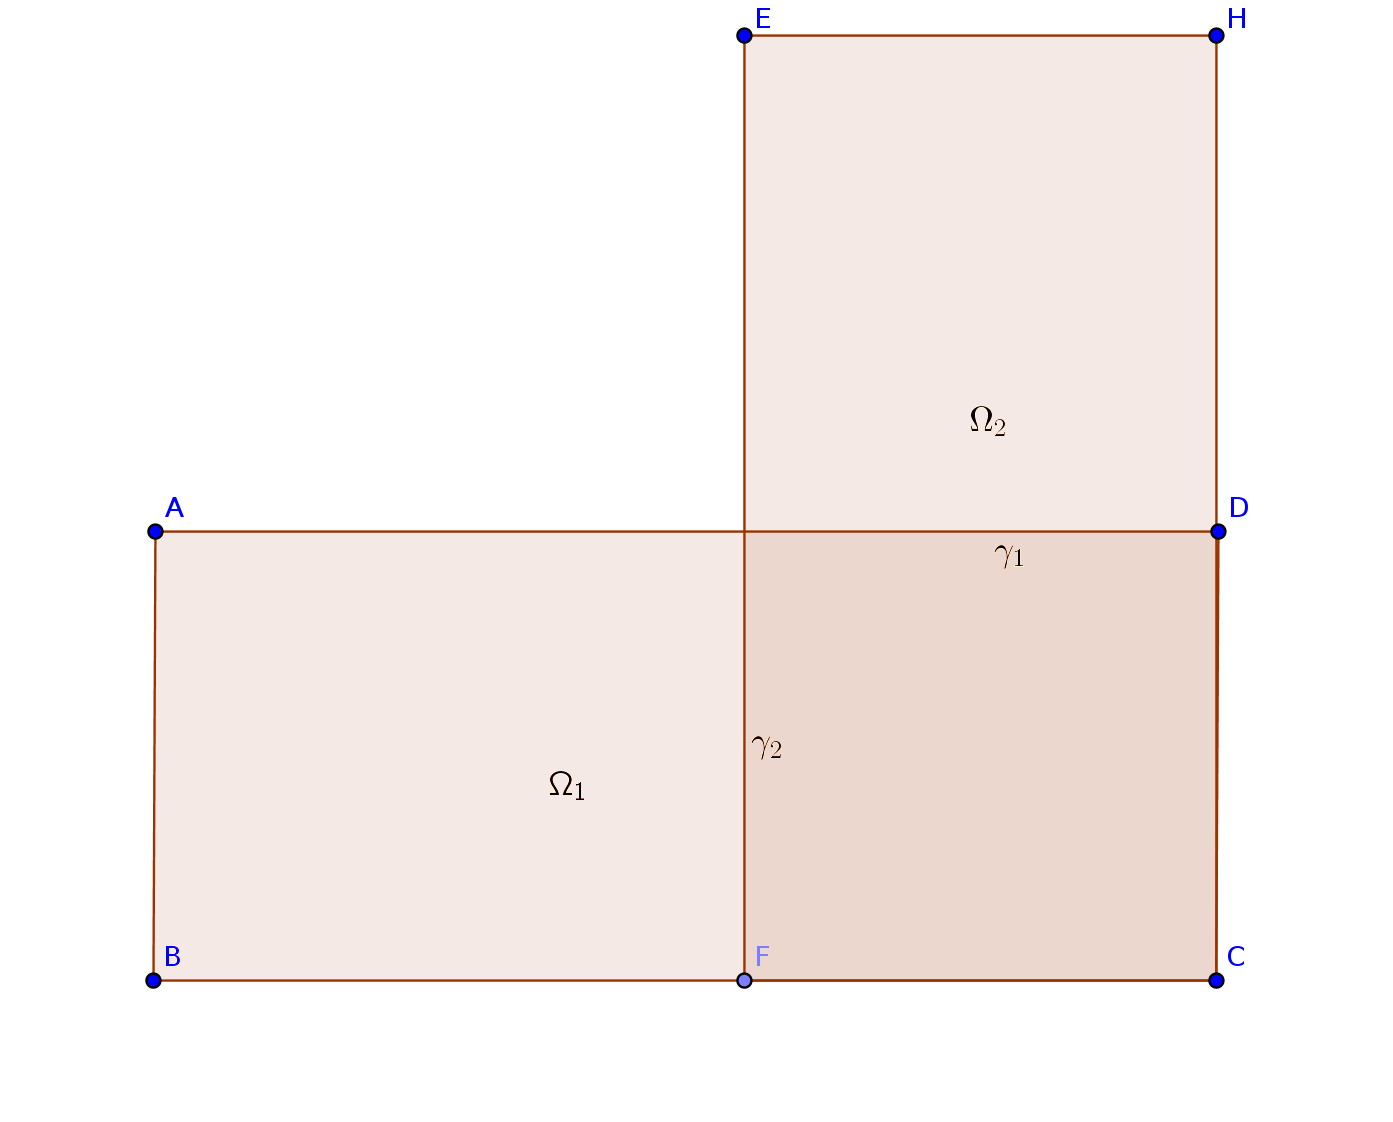
\includegraphics[width=140mm,scale=0.4]
{lshapedomain.png}
\end{figure}
We first show that $Y=Y_1+Y_2$ is a proper subspace of $X$. Assume for contradiction that $X=Y_1+Y_2$, then for each $u\in X$, we have $u=u_1+u_2$ where $u_1\in Y_1$, $u_2\in Y_2$. Now we consider the trace defined as
$$\mathrm{Tr}\colon H^{1} \to H^{\frac{1}{2}}(\partial \Omega).$$
Since $u\equiv 1\in H^1(\Omega)$ and $u$ is continuous on $\overline{\Omega}$, then 
$$1=\mathrm{Tr}u=\mathrm{Tr}(u_1+u_2)=\mathrm{Tr}u_1+\mathrm{Tr}u_2.$$

We also have $\mathrm{Tr}u_1=0$ on $\partial\Omega_1$, and $\mathrm{Tr}u_2=0$ on $\partial\Omega_2$, so $\mathrm{Tr}u_2=1$ on $\gamma_1$ and $\mathrm{Tr}u_1=1$ on $\gamma_2$. This implies that $\mathrm{Tr}u_1=\mathbbm{1}_{\gamma_2}$ on $\gamma_1\cup\gamma_2$, but $\mathbbm{1}_{\gamma_2}\notin H^{\frac{1}{2}}(\gamma_1\cup\gamma_2)$ as
$$\int_{(\gamma_1\cup\gamma_2)}\int_{(\gamma_1\cup\gamma_2)}\frac{|\mathbbm{1}_{\gamma_2}(x)-\mathbbm{1}_{\gamma_2}(y)|^2}{|x-y|} dx dy=\infty,$$
thus yields a contradiction.

\par
Now we proceed to the density argument. Note that for each $u\in Y=Y_1+Y_2$, for $\varepsilon>0$,  there exists $\varphi_i\in Z_i$ such that $$\|u-\varphi_1-\varphi_2\|_{H^1}<\varepsilon.$$ Define
$Z:=\{\varphi \in C^{\infty}(\Omega)\colon \varphi=0 \mbox{ near the problematic point}\}$, then $Z=Z_1+Z_2$.
 It suffices to show that for each $u\in C^{\infty}(\Omega)$, for all $\varepsilon>0$, there exists $\varphi\in Z$ such that $\|u-\varphi\|_{H^1}<\varepsilon$. Assume that $z$ is the probematic point, and consider the function $\varphi_{\varepsilon}\colon \Omega\to\mathbb{C}$ defined as 
$$\varphi_{\varepsilon}(x,y)=\begin{cases} \left(\frac{|(x,y)-z|}{\varepsilon}\right)^{\varepsilon}, \mbox{ for } r=|(x,y)-z|\in(0,\varepsilon), \\
1,  \mbox{ otherwise}.\\
\end{cases}$$
For each $u\in C^{\infty}(\Omega)$, we have $u_{\varepsilon}:=u\cdot \varphi_{\varepsilon}\in \tilde{Z}:=\{\varphi\in C^1(\Omega),\varphi=0 \mbox{ near the problematic point}\}$. Since $Z$ is dense in $\tilde{Z}$, it suffices to show that $\|u-u_{\varepsilon}\|_{H^1}\to 0$ as $\varepsilon\to\infty$. Note that
$$\|u-u_{\varepsilon}\|_{L^2}\rightarrow 0 \mbox{ as } \varepsilon\rightarrow 0,$$ and 
\begin{align*}
\|\bigtriangledown u-\bigtriangledown u_{\varepsilon}\|_{L^2}&=\| \bigtriangledown u (1-\varphi_{\varepsilon})-u\bigtriangledown \varphi_{\varepsilon}\|_{L^2}\\
{}&\leq C(\|1-\varphi_{\varepsilon}\|_{L^2}+\|\bigtriangledown \varphi_{\varepsilon}\|_{L^2})
\end{align*}
for some positive constant $C$. It is obvious that $\|1-\varphi_{\varepsilon}\|_{L^2}\to 0$ as $\varepsilon\to 0$.
Also,
\begin{align*}
\|\bigtriangledown\varphi_{\varepsilon}(x,y)\|_{L^2}&=\| \bigtriangledown \varphi_{\varepsilon}(r)\|_{L^2}\\
{}&= \| \left(\frac{r}{\varepsilon}\right)^{\varepsilon-1}(\cos\theta, \sin\theta)\|_{L^2}\\
{}&=\left(\int_{0}^{\varepsilon}\int_{0}^{2\pi} \left(\frac{r}{\varepsilon}\right)^{2\varepsilon-2} r dr d\theta\right)^{\frac{1}{2}}\\
{}&=\sqrt{2\pi}\left(\int_{0}^{\varepsilon}\left(\frac{r}{\varepsilon}\right)^{2\varepsilon-2} r dr\right)^{\frac{1}{2}}\\
{}&=\sqrt{2\pi} \sqrt{\frac{\varepsilon}{2}}\\
{}&=\sqrt{\pi \varepsilon}
\end{align*}
tends to $0$ as $\varepsilon\to 0$.
Thus, $\|u-u_{\varepsilon}\|_{H^1}=\|u-u_{\varepsilon}\|_{L^2}+\|\bigtriangledown  u-\bigtriangledown u_{\varepsilon}\|_{L^2}\to 0$ as $\varepsilon\to 0$.
\end{proof}
\end{lemma}

